\documentclass{templateppgmo}
% Documento utilizando a classe template da PPGMO

%==============================================================================
% Pacotes usados no documento
%==============================================================================

% Pacote para desenhos gráficos
\usepackage[all,knot,arc,import,poly]{xy}
% Este pacote pode conflitar com outros pacotes gráficos como o ``pictex''
% Então é necessário usar apenas um dos pacotes conflitantes

% Pacotes para inclusão de tabelas
\usepackage{tabularx}
\usepackage{array}

% Pacotes para ambientes matemáticos
\usepackage{amsfonts, amsmath, amssymb}

% Pacote para escrever algoritmos em pseudo-código
\usepackage{algpseudocode}

% Pacote para formatação de diversos códigos fontes
\usepackage{listings}

\usepackage{color}

\usepackage{lipsum}

%numerar as figuras, tabelas e quadros conforme a seção
\numberwithin{figure}{chapter}
\numberwithin{table}{chapter}
\numberwithin{quadro}{chapter}
\numberwithin{algoritmo}{chapter}
\numberwithin{codigo}{chapter}

%==============================================================================
% Configurações dos dados do documento
%==============================================================================

% Título do trabalho
\titulo{Template para Estudo Dirigido I e II do Mestrado em Modelagem e Otimização}

% Nome do autor, entre colchetes se coloca a forma com que geralmente seu nome aparece em citações.
\autor[Sobrenome, Inicias do nome]{Nome do autor}{Sobrenome}

% Define o nome da instituição
\instituicao{Universidade Federal de Goiás -- Regional Catalão}

% Define o local
\local{Catalão -- GO}

% Nome do Orientador, se for orientadora: substitua Orientador por Orientadora no Colchetes
\orientador[Orientador]{Nome do orientados }{Sobrenome}

% Nome do Coorientador (caso não exista basta comentar com %)
%\coorientador[Coorientador]{Nome da Coorientadora}

% Nome do departamento
\departamento{Unidade Acadêmica Especial de Matemática e Tecnologia}

% Área de concentração do trabalho
\area{Modelagem e Otimização}

% Modalidade do curso, nome do curso e grau obtido
\curso{Programa de Pós-Graduação}{Modelagem e Otimização}{Mestre}

% Membros da banca examinadora
% - O primeiro membro será automaticamente o orientador
% - Caso haja coorientador, este será o segundo membro
% Nome dos demais membros e suas instituições
%\membrobanca{Nome do Primeiro Avaliador}{Instituição}
%\membrobanca{Nome dos Segundo Avaliador}{Instituição}

% Data da defesa
\data{20}{março}{2015} %Dia, mês e ano.



%==============================================================================
% Configuração dos elementos pré-textuais
%==============================================================================


% Resumo
\textoresumo{
Este trabalho é um breve modelo de um relatório de estudo dirigido utilizando o ambiente \LaTeX. Para a confecção deste modelo foi utilizado o pacote de classes \textit{ABNTex2} que segue as normas da Associação Brasileira de Normas Técnicas. A elaboração de uma monografia pode ser feita sobrescrevendo o conteúdo deste modelo. Evitar o uso de abreviaturas, símbolos, fórmulas, equações e citações no resumo. Deve ter pelo menos 4 palavras-chave}



% Palavras chaves
\palavrachave{Primeira Palavra Chave}
\palavrachave{Segunda Palavra Chave}
\palavrachave{Terceira Palavra Chave}
\palavrachave{Quarta Palavra Chave} %Insira quantas julgar necessárias


% \textoabstract{
% Abstract text - deve seguir as mesmas orientações do resumo, com pelo menos 4 palavras-chaves
% }

% \keyword{First keyword}
% \keyword{Second keyword}
% \keyword{Third keyword }
% \keyword{Fourth keywrod } %Insira quantas julgar necessárias




%==============================================================================
% Comandos definidos para este documento
%==============================================================================

% Comando simples para exibir comandos Latex no texto
\newcommand
{\comando}[1]{\textbf{$\backslash$#1}}


%==============================================================================
% Início do documento
%==============================================================================
\makeatletter
\newcommand{\fakefloat}[2]{\begingroup\df\@captype{#1}#2\endgroup}
\makeatother
\DeclareOldFontCommand{\it}{\normalfont\itshape}{\mathit}


%%%indicar o tipo de trabalho
%Estudo Dirigido 1 = 1
%Estudo Dirigido 2 = 2
%
\tipodetrabalho{1}

\begin{document}

\chapter{INTRODUÇÃO \label{capitulo:introducao}}

%\addcontentsline{toc}{chapter}{INTRODUÇÃO}

\textual 

Este documento explica brevemente como trabalhar com o \emph{template} desenvolvido pelo programa de pós-graduação em modelagem e otimização (PPGMO)\sigla{PPGMO}{Programa de pós-graduação em Modelagem e Otimização} para confeccionar o relatório de estudo dirigido em \LaTeX seguindo as normas da Associação Brasileira de Normas Técnicas (ABNT)\sigla{ABNT}{Associação Brasileira de Normas Técnicas} e o \textit{Guia Para Apresentação de Trabalhos Acadêmicos na UFG}~\cite{mendonca:2005,mendonca:2006}. O \emph{template} foi devidamente aprovação pelo colegiado do PPGMO da Unidade Acadêmica Especial de Matemática e Tecnologia (IMTec)\sigla{IMTec}{Unidade Acadêmica Especial de Matemática e Tecnologia} da Regional Catalão (RC) \sigla{RC}{Regional Catalão} da Universidade Federal de Goiás (UFG)\sigla{UFG}{Universidade Federal de Goiás}.

O \emph{template} foi construído com base na classe \textit{abntex2} mantendo as mesmas opções presentes nesta classe, portanto é recomendável que seja consultada a documentação do \textit{abntex2}. A classe AbnTex2 foi desenvolvida para facilitar a produção em \LaTeX  de documentos seguindo as normas da ABNT~\cite{araujo:2015:classe_abnt2}.

O requisito básico para utilização do \emph{template} é criar um documento desta classe com o comando
\comando{documentclass\{templateppgmo\}}.



\chapter{ABNT E TRABALHOS ACADÊMICOS \label{capabnt}}

Segundo a ABNT NBR 14724:2011, seção 4.2.2, ``o texto é composto de uma parte introdutória, que apresenta os objetivos do trabalho e as razões de sua elaboração; o desenvolvimento, que detalha a pesquisa ou estudo realizado; e uma parte conclusiva.''

Os títulos dos capítulos textuais são à critério do autor e não há nenhuma normatização a respeito deles. No entanto, geralmente o capítulo “Introdução” e o capítulo “Conclusão” (ou “Considerações finais”) são, respectivamente, o primeiro e o último capítulo textual.

É importante destacar que a norma em tela e a ABNT NBR 6024:2012 não são explícitas sobre a possibilidade de não numeração de capítulos textuais. 

Deve constar na introdução:
- Delimitação do assunto tratado;
- Objetivos da pesquisa;
- Outros elementos necessários para situar o tema do trabalho.

Segundo as Resolução que disciplina o Estudo Dirigido, o relatório deverá ser apresentado conforme o esse modelo, assim contendo:

\begin{itemize}

\item Capa (em 1 página): deve conter o nome da universidade, o nome do programa, o título do relatório, a identificação do aluno, a identificação do professor orientador e o ano.
\item Resumo e palavras-chave (em 1 página)
\item Sumário (em 1 página)
\item Introdução: deve caracterizar o objeto de estudo, descrevendo, de forma sucinta, o(s) problema(s) abordado(s), o(s) objetivo(s) pretendido(s) e a(s) justificativa(s). 
\item Desenvolvimento: deve descrever o trabalho realizado, incluindo a revisão bibliográfica, os métodos, recursos e técnicas utilizadas para lidar com o problema proposto, bem como os resultados já alcançados. Pode ser colocado em mais de um capítulo.
\item Conclusões
\item Bibliografia: deve apresentar as fontes consultadas e citadas, conforme as normas da ABNT – Associação Brasileira de Normas Técnicas.
\item Apêndices e Anexos: se existentes, devem apresentar material complementar cujo conteúdo é mencionado no corpo do relatório e que possa ser consultado para melhor entendimento do texto.

\end{itemize}

É interessante observar que a ABNT NBR 14724:2011 recomenda que os documentos sejam impressos no anverso e no verso das folhas. 


%%%NOVO CAPÍTULO
\chapter{INSERÇÃO DE DADOS PRÉ-TEXTUAIS \label{capinsercao}}

No \emph{templateppgmo} a configuração de diversas opções e principalmente dos elementos pré-textuais é realizada com comandos específicos inseridos antes de \comando{begin\{document\}}.

Os principais comandos do \emph{template} são:

\begin{description}
\item[\comando{titulo\{T\}}] Título do trabalho (substitua T pelo título do trabalho);
\item[\comando{autor[A]\{N\}}] Nome do autor do trabalho, onde N é o nome do autor e A é forma empregada pelo autor em suas publicações;
\item[\comando{orientador\{O\}}] Nome do professor orientador do trabalho. Caso seja uma orientadora pode ser usado o comando \comando{orientador[Orientadora:]\{O\}} (sendo que O deve ser substituído pelo nome do orientador ou orientadora);

\item[\comando{data\{Dia\}\{Mês\}\{Ano\}}] Data da defesa da dissertação. Dia com dois dígitos, Mês por extenso e ano com 4 dígitos.

\end{description}

Para inclusão dos demais campos pré-textuais o mestrando deve preencher os seguintes campos:

\begin{description}


\item[\comando{textoresumo\{
inserção do resumo\}}]
\item[\comando{palavrachave\{Primeira Palavra Chave\}}]
\item[\comando{palavrachave\{Segunda Palavra Chave\}}]
\item[\comando{palavrachave\{Terceira Palavra Chave\}}]
\item[\comando{palavrachave\{Quarta Palavra Chave\}}]
Insira quantas palavras-chave julgar necessárias, com no mínimo 4.


Neste caso é preciso executar o comando para gerar a lista de siglas na ordem correta:
\begin{itemize}
\item pdflatex
\item pdflatex
\item makeindex monografia.nlo -s nomencl.ist -o monografia.nls
\item pdflatex
\end{itemize}

\end{description}

%%%%%%Novo capítulo
\chapter{CONFIGURAÇÕES DO DOCUMENTO \label{capconfiguracoes}}

Os que usarão o \emph{templateppgmo} em \LaTeX\; não precisam se preocupar em configurar o layout do documento. O pdf gerado pelo template estará normatizado de acordo com o aprovado pelo colegiado do programa.

Os que forem empregar outro editor de texto, devem configurar tal editor para se ajustar ao padrão do programa.


\section{Fontes e Espaçamento}

\begin{itemize}
\item Fonte tamanho 12.

\item Tipo de fonte Times New Roman

\item Citações de mais de três linhas, notas de rodapé\footnote{Esse é um exemplo de nota de rodapé}, paginação e legendas de ilustrações e tabelas devem ser digitadas em tamanho menor e uniforme (Fonte tamanho 9 em Times New Roman).

\item Espaço entre linhas de 1,5.

\item Citações de mais de três linhas, notas de rodapé, referências, legendas, natureza do trabalho, objetivo, nome da instituição e área de concentração em espaço simples entre linhas.

\item Dois espaços de 1,5 linhas entre títulos e texto. 

\item Um espaço de 1,5 linhas entre equação/fórmula e texto, antes e depois.

\item Títulos com indicativos numéricos: alinhados à esquerda.

\item Títulos sem indicativos numéricos: centralizados. 

\item Os títulos das secções primárias devem se iniciar em folhas distintas.

\item Todas as folhas do trabalho, após a capa, devem ser contadas sequencialmente, mas não numeradas. 

\item A numeração é colocada a partir da primeira folha da parte textual. 

\item A numeração deve ser em algarismos arábicos, no canto superior direito da folha. 

\item Parágrafo deve ter recuo à esquerda de 1,25cm.

\item O título do capítulo deve aparecer em caixa alta. O primeiro subtítulo deve aparecer com a primeira letra de cada palavra em maiúscula (exceto conectivos, preposições, e palavras com menos de 3 letras). A partir do segundo subtítulo, deve aparecer somente a primeira letra da primeira palavra em maiúscula, sendo as demais todas minúsculas.

\item O relatório deverá conter pelo menos 8 páginas.

\item Para mudar o formato para o Estudo Dirigido 2, substituir o comando \comando{tipodetrabalho\{1\}} por \comando{tipodetrabalho\{2\}}.

\end{itemize}

\section{Margens e Paginação}
As margens devem ser: para o anverso, esquerda e superior de 3 cm e direita e inferior de 2 cm; para o verso, direita e superior de 3 cm e esquerda e inferior de 2 cm.

\subsection{Sobre as folhas}

Todas as folhas do trabalho, a partir da capa, devem ser contadas sequencialmente, mas não numeradas (folhas pré-textuais). A numeração começa a partir da primeira folha de parte textual (Introdução), em algarismos arábicos, no canto superior direito da folha.

\subsubsection{Próximo capítulo}

O próximo capítulo aborda sobre corpos flutuantes.

%novo capítulo
\chapter{CORPOS FLUTUANTES \label{capcorpos}}

Corpos flutuantes são elementos não textuais como figuras e tabelas que complementam as informações do texto. Conforme a ABNT NBR 14724:2011, seção 5.8, o rótulo é atribuído acima do elemento e a legenda abaixo.

\section{Figuras \label{secao:figuras}} 

A inserção de figuras é realizada normalmente através do comando~\comando{begin\{figure\}}. Na Figura \ref{figura:exemplo_grafo} é mostrado um exemplo de grafo com o pacote \textit{xy}. Já a Figura \ref{figura:logomarca_ufg} exibe a logomarca da UFG com o pacote \textit{graphicx}. 

Desde 2012, deve ser incorporado ao corpo flutuante do tipo figura, além da legenda, a fonte de onde esta foi extraída. Se a figura foi confeccionada pelo próprio autor, deve se colocar " o autor". Para citar uma figura: ``a Figura \ref{figura:exemplo_grafo} como do próprio autor''. As Figuras devem ficar centralizadas no texto, assim como o texto do rótulo e da fonte.

\begin{figure}[]
\caption{Exemplo de grafo.}
\label{figura:exemplo_grafo}
\centering
\begin{scriptsize}
$$
\xymatrix@R20pt@C10pt{
& & & & vr \ar[dlll] \ar[dl] \ar[d] \ar[dr] \ar[drr] \ar[drrr] & & & \\
& (a_3, b_2, c_1) \ar[d]^{\varphi_2} \ar[dl]_{\varphi_1} & & (a_3, b_2, c_2) \ar[d]^{\varphi_2} \ar[dl]_{\varphi_1} & (a_1, b_1, c_1) & (a_1, b_1, c_2) & (a_1, b_2, c_1) & (a_1, b_2, c_2) \\
(a_2, b_2, c_1) \ar[dr]_{\varphi_3} & (a_3, b_1, c_1) \ar[d]^{\varphi_1} & (a_2, b_2, c_2) \ar[dr]_{\varphi_3} & (a_3, b_1, c_2) \ar[d]^{\varphi_1} & & & & \\
& (a_2, b_1, c_1)  & & (a_2, b_1, c_2) & & & & \\
}
$$
\end{scriptsize}
\legend{Fonte: o  autor.}
\end{figure}

\begin{figure}[H]
\caption{Logomarca da UFG.}
\label{figura:logomarca_ufg}
\centering

\includegraphics{figuras/prioritaria_tipo1}
\legend{Fonte: Universidade Federal de Goiás.}
\end{figure}


\section{Tabelas \label{secao:tabelas_e_quadros}}

A inserção de tabelas e quadros é feita de forma semelhante a inserção de figuras, porém são utilizados os ambientes \textit{table} e \textit{quadro}. A principal diferença entre tabelas e quadros, de acordo com \citeonline{mendonca:2005}, é que as tabelas são destinadas para informações numéricas e os quadros são mais adequados para informações textuais. Assim como na figura, toda tabela deve conter, além da legenda, a fonte de onde esta foi extraída. Se a tabela foi confeccionada pelo próprio autor, deve se colocar " o autor". Para citar uma tabela no texto, tem-se: ``... a Tabela \ref{tabela:lista_produtos} foi feita pelo próprio autor e mostra uma tabela...''. As Tabelas devem ficar centralizadas no texto, assim como o texto do rótulo e da fonte.

Como exemplos foram inseridas a Tabela \ref{tabela:lista_produtos} que exibe uma de lista de produtos e a Tabela \ref{tabela:populacao_america_sul} que mostra a população dos países da América do Sul. Foi inserido também o Quadro \ref{quadro:editores_texto_livres} com alguns editores que podem ser usados para se trebalhar com Latex para demonstrar a inserção de quadros.




\begin{table}[H]
\centering
\caption{Lista de produtos.}
\label{tabela:lista_produtos}
\begin{tabularx}{\textwidth}{X|l|r|r|r} \hline
Produto      & Unidade & Preço (R\$) & Quantidade & Total (R\$) \\ \hline
Arroz        & Kg      & 2,00        & 550        & 1.100,00    \\
óleo de Soja & L       & 2,50        & 500        & 750,00      \\
Açucar       & Kg      & 3,00        & 100        & 300,00      \\ \hline
\end{tabularx}

\legend{Fonte: o autor.}
\end{table}

\begin{table}[H]
\centering
\caption{População dos países da América do Sul.} \label{tabela:populacao_america_sul}
\begin{tabular}{r|l|r}        \hline
Código  & País            & População   \\ \hline
1       & Brasil          & 191.480.630 \\
2       & Argentina       &  39.934.100 \\
3       & Colômbia        &  46.741.100 \\
4       & Paraguai        &   9.694.200 \\
5       & Uruguai         &   3.350.500 \\
6       & Peru            &  28.221.500 \\
7       & Equador         &  13.481.200 \\
8       & Bolívia         &   9.694.200 \\
9       & Venezuela       &  28.121.700 \\
10      & Chile           &  16.803.000 \\ \hline
\end{tabular}

\legend{Fonte: \citeonline{wikipedia:2011:america_sul}.}
\end{table}

\begin{quadro}[htb]
\centering
\caption{Editores de Texto Livres.} \label{quadro:editores_texto_livres}
\begin{tabular}{|l|l|r|}        \hline
Editor     & Multiplataforma & Específico para Latex \\ \hline
Kwriter    & Sim             & Não                   \\
Texmaker   & Sim             & Sim                   \\
Kile       & Sim             & Sim                   \\
Geany      & Sim             & Não                   \\ \hline
\end{tabular}

\legend{Fonte: o autor.}
\end{quadro}



\section{Tabelas em Formato IBGE}

O template baseado na classe ABNTex prevê inserção de tabelas no formato do IBGE. Vide Tabela~\ref{tabela-ibge}.

\begin{table}[H]
\IBGEtab{%
\caption{Um Exemplo de tabela alinhada que pode ser longa ou curta,
  conforme padrão IBGE.}%
  \label{tabela-ibge}
}{%
\begin{tabular}{ccc}
\toprule
Nome & Nascimento & Documento \\
\midrule \midrule
Maria da Silva & 11/11/1111 & 111.111.111-11 \\
\bottomrule
\end{tabular}%
}{%
  \fonte{Produzido pelos autores}%
  \nota{Esta é uma nota, que diz que os dados são baseados na regressão linear.}%
  \nota[Anotações]{Uma anotação adicional, seguida de várias outras.}%
  }
  \legend{Fonte: IBGE.}
  \end{table}


%novo capítulo
\chapter{ALGORITMOS}

Este capítulo mostra como lidar com algoritmos.

\section{Algoritmos e Códigos}
\label{secao:algoritmos_e_codigos}

Além dos corpos flutuantes convencionais para inserir figuras (\comando{begin\{figure\}}) e tabelas (\comando{begin\{figure\}}), o \emph{templateppgmo} possui mais dois tipos de corpos flutuantes um para algoritmos (\comando{begin\{algoritmo\}}) e outro para códigos (\comando{begin\{codigo\}}). A utilização de um ou de outro fica a critério do usuário. Como exemplo temos o Algoritmo \ref{algoritmo:mdc} que calcula o máximo divisor comum entre dois números e os Códigos \ref{codigo:notas_alunos} e \ref{codigo:metodo_leitura} que são uma consulta na \textit{Structured Query Language (SQL)}\sigla{SQL}{Structured Query Language} e uma sobrotina em \textit{Java}.

\begin{algoritmo}[H]
\begin{algorithmic}[1]
\Require Dois números inteiros ($n_1, n_2$)
\If{$n_2 > n_1$} \Comment{Garante que o maior número seja $n_1$}
\State troca valores de $n_1$ e $n_2$
\EndIf
\Repeat
\State $r \leftarrow$ resto da divisão de $n_1$ por $n_2$
\State $n_1 \leftarrow n_2$
\State $n_2 \leftarrow r$
\Until{$r > 0$}
\Return $n_1$
\end{algorithmic}
\caption{Algoritmo para cálculo de máximo divisor comum MDC($n_1$,$n_2$).}
\label{algoritmo:mdc}
%\legend{Fonte: o autor.}

\end{algoritmo}


Existem diversos outros pacotes disponíveis para escrever algoritmos e códigos. Nos exemplos anteriormente foram utilizados o pacote \textit{algpseudocode} e \textit{listings}. O pacote \textit{algpseudocode} é usado para escrever algoritmos em alto nível \cite{janos:2005:algpseudocode}. Já o pacote \textit{listings} serve para escrever os códigos em diversas linguagens de programação \cite{moses:2006:listings}. 


\begin{codigo}[H]
\lstset{language=SQL, breaklines=true}
\begin{lstlisting}
SELECT a.nome_aluno AS aluno,
d.nome_disciplina AS disciplina,
m.nota AS nota
FROM aluno AS a,
disciplina AS d,
matriculado AS m
WHERE a.id_aluno = m.id_aluno
AND d.id_disciplina = m.id_disciplina
ORDER BY a.nome_aluno, d.nome_disciplina;
\end{lstlisting}
\caption{Consulta SQL.}
\label{codigo:notas_alunos}
%\legend{Fonte: o autor.}
\end{codigo}

\begin{codigo}[H]
\lstset{language=Java, breaklines=true}
\begin{lstlisting}
public static String Leitura(){
	BufferedReader reader = new BufferedReader(new InputStreamReader(System.in));
	try {
		return reader.readLine(); // Le uma linha pelo teclado
		} catch (IOException e) {
			e.printStackTrace();
			return "";
		}
	}
	\end{lstlisting}
	\caption{Subrotina para obter uma entrada do usuário.}
	\label{codigo:metodo_leitura}
	%\legend{Fonte: adaptado de \cite{araujo:2015:classe_abnt2}.}
	\end{codigo}

	
	

  	%%%novo capítulo
  	\chapter{AMBIENTES MATEMÁTICOS}

  	Os seguintes ambientes matemáticos foram inseridos no template:
  	\begin{itemize}
  	\item Teoremas (\comando{begin\{teorema\}[\ ]} ... \comando{begin\{teorema\}});
  	\item Proposição (\comando{begin\{proposicao\}[\ ]} ... \comando{begin\{proposicao\}});
  	\item Lema (\comando{begin\{lema\}[\ ]} ... \comando{begin\{lema\}});
  	\item Corolário (\comando{begin\{corolario\}[\ ]} ... \comando{begin\{corolario\}});
  	\item Exemplo (\comando{begin\{exemplo\}[\ ]} ... \comando{begin\{exemplo\}});
  	\item Observação (\comando{begin\{observacao\}[\ ]} ... \comando{begin\{observacao\}});
  	\item Definição (\comando{begin\{definicao\}[\ ]} ... \comando{begin\{definicao\}});
  	\item Demonstracao (\comando{begin\{demonstracao\}[\ ]} ... \comando{begin\{demonstracao\}}).
  	\end{itemize}

  	Abaixo temos um exemplo de proposição com sua demonstração:
  	\begin{proposicao}
  	Sejam $a$ e $b$ reais, tais que $0<a<b$. Então $a^2<b^2$.
  	\end{proposicao}

  	\begin{demonstracao}[Prova direta]
  	Pela hipótese concluímos que $(b+a)>0$ e $(b-a)>0$.

  	Como $b^2-a^2=(b+a)(b-a)$ concluímos que $b^2-a^2>0$, ou seja, $a^2<b^2$.
  	\end{demonstracao}

  	Neste documento tratamos brevemente apenas dos ambientes mencionados anteriormente. Contudo, para escrever expressões matemáticas complexas é preciso estudar uma documentação mais específica como em \citeonline{cassagojr:1997:amslatex}.


  	As equações/fórmulas podem ser inseridas no documento fazendo:

  	\begin{itemize}
  	\item Teoremas (\comando{begin\{equation\}[\ ]} ... \comando{begin\{equation\}});
  	\end{itemize}

  	Por exemplo, para referenciar uma equação, tem-se o exemplo: ``Conforme a eq. (\ref{eq1}), chega-se no número médio para...''. 

  	\begin{equation} \label{eq1}
  	\displaystyle \sum_{j \in A} x_j + \int x^2  + f(z) 
  	\end{equation}

  	Observe que a equação aparece centralizada e com numeração entre parênteses, alinhada a direita, e referenciada pelo número do capítulo seguido pelo número da respectiva equação dentro daquele capítulo.


  	%novo capítulo
  	\chapter{FERRAMENTAS ÚTEIS}
  	\label{capitulo:ferramentas_uteis}

  	Existem diversas ferramentas para se trabalhar com \LaTeX. Duas ferramentas que merecem destaque são o editor \textit{Texmaker} exibido na Figura \ref{figura:texmaker} e o gerenciador de referências \textit{JabRef} mostrado na Figura \ref{figura:jabref}. Ambas ferramentas são livres e multiplataforma.

  	\begin{figure}[H]
  	\caption{Tela do Texmaker.}
  	\label{figura:texmaker}
  	\centering
  	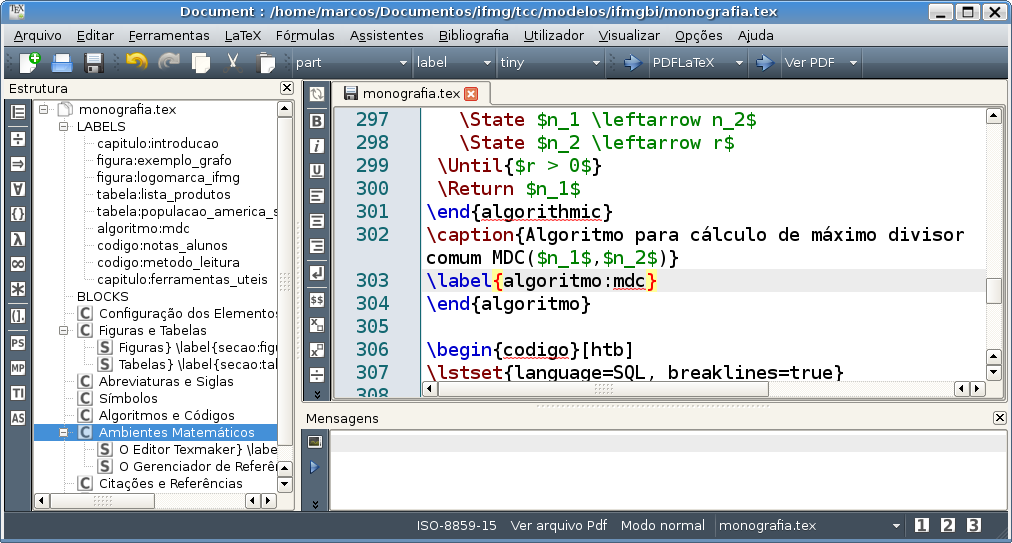
\includegraphics[scale=.3]{figuras/texmaker}
  	\legend{Fonte: o autor.}
  	\end{figure}

  	\begin{figure}[H]
  	\caption{Tela do JabRef.}
  	\label{figura:jabref}
  	\centering
  	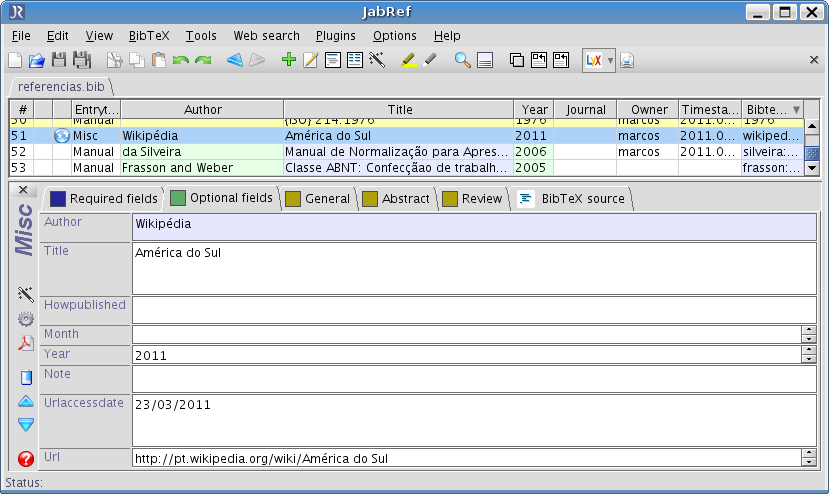
\includegraphics[scale=.3]{figuras/jabref}
  	\legend{Fonte: o autor.}
  	\end{figure}



  	O Texmaker pode ser obitido em \url{www.xm1math.net/texmaker} e o JabRef pode ser obtido em \url{jabref.sourceforge.ne}. é importante ressaltar que o Texmaker é apenas um editor, para compilar os documentos é necessário que o  \LaTeX \; esteja instalado. Os ambientes \LaTeX \; mais populares são o Texlive (\url{www.tug.org/texlive}) e o MiKTex (\url{miktex.org}).


  	\chapter{CITAÇÕES E REFERÊNCIAS}

  	O \emph{template} foi confeccionado de forma a facilitar a compilação das referencias via BibTeX. 

  	Basta, portanto, que seja incluso o nome do arquivo .bib no comando:

  	\comando{bibliography\{<nome do aquivo bib>\}}. 

  	Neste texto as referencias foram inseridas no arquivo referencias.bib. Assim, foi utilizado o comando \comando{bibliography\{referencias\}} para associar o arquivo bib ao documento. Para compilar a bibliografia deve se executar os seguintes comando \LaTeX \; 

  	\begin{itemize}
  	\item pdflatex monografia.tex
  	\item pdflatex monografia.tex
  	\item bibtex monografia
  	\item pdflatex monografia.tex
  	\end{itemize}

  	\section{Informações Úteis sobre Citações e Referências}

  	Em documentos acadêmicos podem existir citações diretas e citações indiretas. As citações indiretas são feitas quando se reescreve uma referência consultada. Nas citações indiretas há duas formatações possíveis dependendo de como ocorre a citação no texto. Quando o autor é mencionado explicitamente  deve ser usado o comando \comando{citeonline\{\}}, nas demais situações é usado o comando \comando{cite\{\}}.

  	\begin{exemplo}
  	Para se gerar o texto:

  	Segundo \citeonline{mendonca:2005}, o trabalho de conclusão de curso deve seguir as normas da ABNT.

  	O código \LaTeX \;é:
  	Segundo \comando{citeonline{\{$\{mendonca:2005\}$}}, o trabalho de conclusão de curso deve seguir as normas da ABNT.

  	\end{exemplo}


  	Para especificar a página consultada na referência é preciso acrescentá-la entre colchetes com os comandos \comando{cite[página]\{\}} ou \comando{citeonline[página]\{\}}. 


  	\begin{exemplo}

  	Para se gerar o texto: 

  	A folha de aprovação é um elemento obrigatório na monografia de projeto final de curso trabalho de conclusão de curso.  \cite[p.~10]{mendonca:2005}.

  	O código \LaTeX \;é:
  	A folha de aprovação é um elemento obrigatório no trabalho de conclusão de curso.  \comando{cite[p.~10]\{ mendonca:2005\} }.

  	\end{exemplo}

  	As citações diretas acontecem quando o texto de uma referência é transcrito literalmente. As citações diretas são curtas (até três linhas) são inseridas no texto entre aspas duplas. 

  	\begin{exemplo}
  	Para se gerar o texto:

  	``Os quadros, ao contrario das tabelas, apresentam dados textuais e devem localizar-se o mais proximo do texto a que se referem'' \cite[p.~25]{mendonca:2005}.

  	O código \LaTeX \; é:
  	``Os quadros, ao contrário das tabelas, apresentam dados textuais e devem localizar-se o mais próximo do texto a que se referem'' \comando{cite[p.~25]\{mendonca:2005\}}.

  	\end{exemplo}

  	As citações longas (com mais de 3 linhas) podem ser inseridas via \comando{begin\{citacao\}} .


  	\begin{exemplo}
  	Com os comandos a seguir:

  	\comando{begin\{citacao\}}
  	Síntese final do trabalho, a conclusão constitui-se de uma resposta à hipótese enunciada na introdução. O autor manifestará seu ponto de vista sobre os resultados obtidos e sobre o alcance dos mesmos. Não se permite a inclusão de dados novos nesse capítulo nem citações ou interpretações de outros autores \comando{cite[p.~25]\{mendonca:2005\}}.
  	\comando{end\{citacao\}}

  	Se produz o seguinte:

  	\begin{citacao}
  	Síntese final do trabalho, a conclusão constitui-se de uma resposta à hipótese enunciada na introdução. O autor manifestará seu ponto de vista sobre os resultados obtidos e sobre o alcance dos mesmos. Não se permite a inclusão de dados novos nesse capítulo nem citações ou interpretações de outros autores \cite[p.~25]{mendonca:2005}.
  	\end{citacao}

  	\end{exemplo}


  	Veja a diferença em citar explicitamente, em que a primeira letra vem em maiúscula, enquanto que implicitamente (entre parênteses), todo o nome vem em maiúsculo. 


  	\section{Outros Modelos de Citação e Forma de Referência}

  	Outros exemplos de citação são dados a seguir, primeiro para o caso explícito e, no final, para o caso implícito. Veja no Capítulo de referências, a forma correta de referenciar cada caso.

  	\begin{itemize}
  	\item Artigo em revista\footnote{obra com quatro ou mais autores têm a referência dos autores apenas com o primeiro seguido de \textit{et al.}}: Segundo o \citeonline{silva:artigo} e \citeonline{artigo1} tem-se.... \cite{silva:artigo,artigo1};

  	\item Artigo em coletânea: Segundo o \citeonline{silva:incollection} tem-se.... \cite{silva:incollection};

  	\item Anais de evento: Segundo o \citeonline{silva:inproceedings} tem-se.... \cite{silva:inproceedings};

  	\item Relatório técnico: Segundo o \citeonline{silva:tech} tem-se.... \cite{silva:tech};

  	\item Monografia: Segundo o \citeonline{silva:monography} tem-se.... \cite{silva:monography};

  	\item Dissertação de mestrado: Segundo o \citeonline{silva:master} tem-se.... \cite{silva:master};

  	\item Tese de doutorado: Segundo o \citeonline{barcelos1998} tem-se.... \cite{barcelos1998};

  	
  	\item Livro: Segundo o \citeonline{wazlawick:2009} tem-se.... \cite{wazlawick:2009};


  	\item Capítulo de livro: Segundo o \citeonline{silva:inbook} tem-se.... \cite{silva:inbook};

  	\item Livreto (livro de brochura)\footnote{este é um exemplo de obra com três autores}: Segundo o \citeonline{silva:booklet} tem-se.... \cite{silva:booklet};

  	\item Manual (documentação técnica, normas...): Segundo o \citeonline{silveira:2006:manual_tcc} tem-se.... \cite{NBR6023:2000};

  	\item Patente: Segundo o \citeonline{cruvinel1989} tem-se.... \cite{cruvinel1989};
  	%\item Páginas de Internet\footnote{pode-se usar o tipo Miscelânea para isto também}: Segundo o \citeonline{marcos:site} tem-se.... \cite{marcos:site};

  	\item Miscelânea\footnote{quando nada se encaixar nas opções conhecidas, como páginas de Internet consultadas}: Segundo o \citeonline{araujo:2015:classe_abnt2} tem-se.... \cite{araujo:2015:classe_abnt2};

  	\item Citações implícitas (entre parênteses) que contam com mais de um trabalho deve vir como o exemplo. Veja o caso de 3 trabalhos sendo citados ao mesmo tempo: A pesquisa da vida conta com tudo \cite{silva:incollection,silva:artigo, cruvinel1989}.

  	\end{itemize}

  	Observar no Capítulo de referências que quando existe obras com o mesmo autor, omite-se o nome do autor (ou autores) nas obras subsequentes. Veja o caso da referência para \citeonline{mendonca:2005}, em que foi listado o nome do autor. Porém, em \citeonline{mendonca:2006}, o nome do autor não aparece, aparecendo apenas ``\_\_\_\_\_\_\_.'', pois é o mesmo autor para diferentes obras.

  	Para cada um dos exemplos acima, veja como a referência foi criada lá no capítulo contendo as referências do trabalho. Deve-se seguir rigorosamente o formato das referências e citações expressas neste documento. Caso a opção desejada não esteja nas referências, use algum dos modelos disponíveis na Seção 8 do documento:

  	http://tug.ctan.org/macros/latex/contrib/abntex2/doc/abntex2cite.pdf

  	Outro documento que pode ser usado é o Capítulo 5 de:

  	https://unoeste.br/site/biblioteca/documentos/Manual-Normalizacao.pdf


  	%novo capítulo
  	\chapter{CONCLUSÕES E TRABALHOS FUTUROS}


  	A conclusão!! Escreva aqui.

  	Como trabalhos futuros, tem-se:
  	\begin{itemize}
  	\item correr bastante;
  	\item ir a luta;
  	\item viver bem.
  	\end{itemize}



  	\postextual
  	\printindex

  	\bibliography{referencias}

  	\apendices

  	\chapter{A VIDA NOTURNA}

  	Para inserir apêndices, basta incluir um novo capítulo abaixo da linha \comando{apendices}.




  	\anexos

  	\chapter{O ANEXO DA VIDA}

  	Para inserir anexos, basta incluir um novo capítulo abaixo da linha \comando{anexos}. 



  	\end{document}

